\documentclass{article}
\usepackage[utf8]{inputenc}
\usepackage{float}
\usepackage{graphicx}

\title{Database II Praktikum Apex} 
\author{Muhammad Wahyu Ardi Ismail \\1184059 \\D4 TI 2B }
\date{November 2019}

\graphicspath{{gambar/}}

\begin{document}

\maketitle

\newpage

\section{Oracle Apex}
\subsection{Pengertian Oracle Apex}
\par Oracle Apex adalah suatu platform pengembangan kode rendah yang memungkinkan anda membangun sebuah aplikasi perusahaan yang dapat diskalakan dan aman dengan fitur \textit{world-class} yang dapat digunakan perangkat lunak apapun. Oracle apex juga merupakan lingkungan pengembangan perangkat
lunak berbasis web yang berjalan pada \textit{database}.

\subsection{Buat Akun Orcale Apex}
\begin{enumerate}
\item pertama buka link https://apex.oracle.com/en/
\item kemudian klik \textit{sign in}

    \begin{figure}[ht]
        \centerline{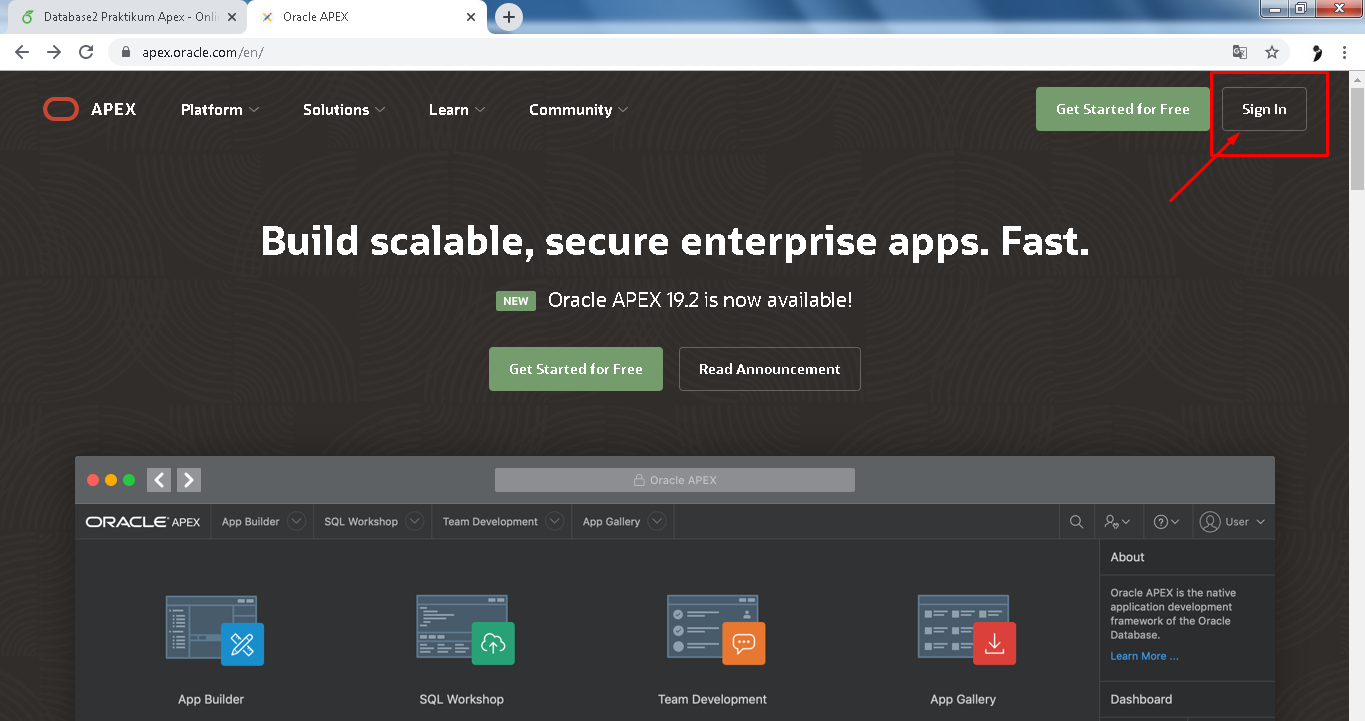
\includegraphics[width=6cm]{a.png}}
        \caption{klik \textit{sign in}}
    \end{figure}

\item kemudian klik \textit{request a work space}

    \begin{figure}[ht]
        \centerline{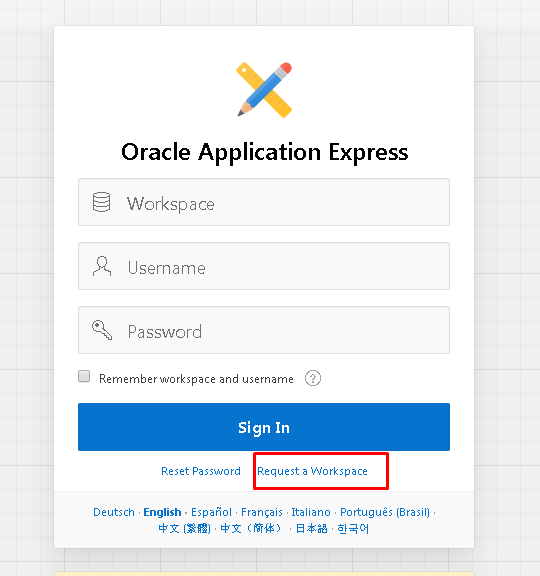
\includegraphics[width=6cm]{b.png}}
        \caption{klik \textit{request a work space}}
    \end{figure}
    
\item kemudian isi data seperti gambar dibawah ini, kemudian klik \textit{next}
    \begin{figure}[ht]
        \centerline{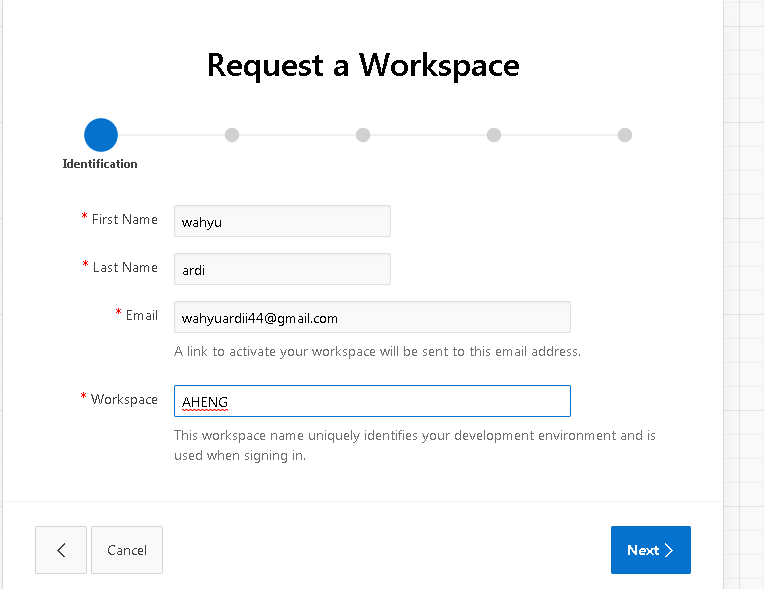
\includegraphics[width=4cm]{c.png}}
        \caption{isi data}
    \end{figure}
    
\item kemudian pilih, jika sudah \textit{next}
    \begin{figure}[ht]
        \centerline{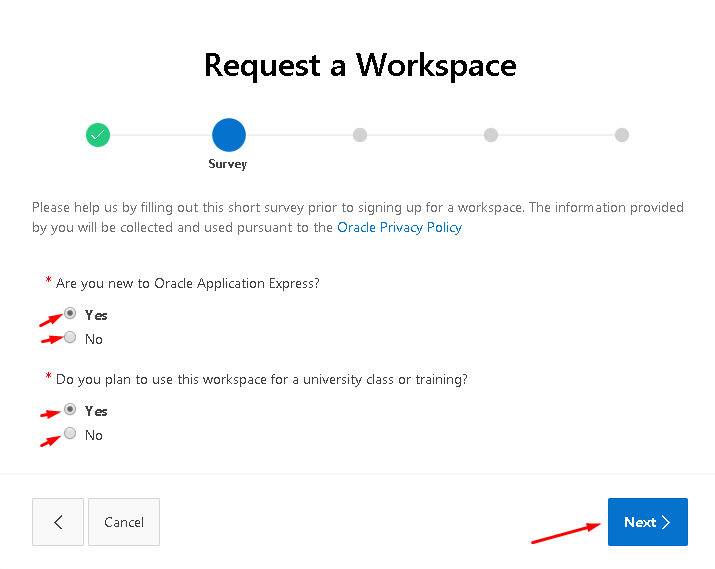
\includegraphics[width=4cm]{d.png}}
        \caption{pilih}
    \end{figure}

\item isi alasan, kemudian klik \textit{next}
    \begin{figure}[ht]
        \centerline{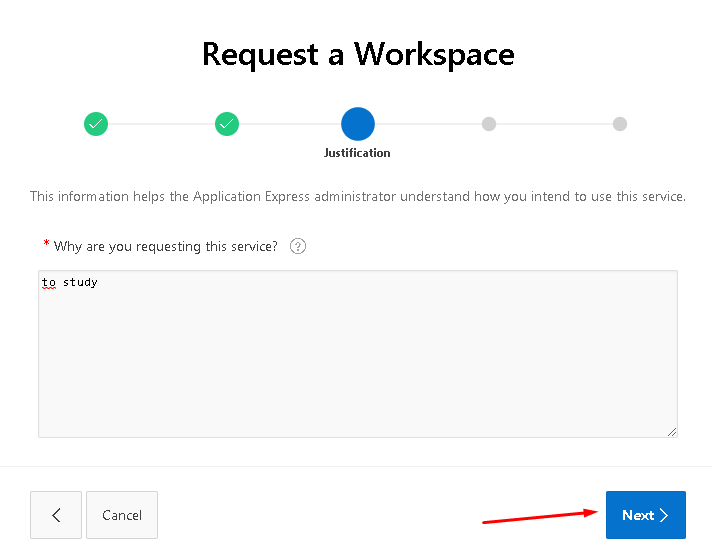
\includegraphics[width=4cm]{e.png}}
        \caption{isi alasan}
    \end{figure}
    
\newpage

\item \textit{request workspace} pilih \textit{i accept the terms} kemudian klik \textit{next}
     \begin{figure}[htb]
        \centerline{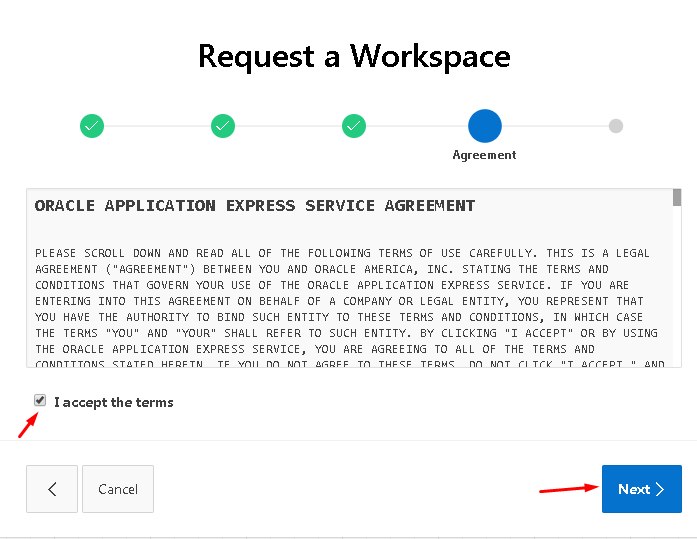
\includegraphics[width=5cm]{f.png}}
        \caption{\textit{request workspace}}
    \end{figure} \\
    
    \item berikut tampilan \textit{confirmation}, jika sudah benar klik \textit{submit request}
    \begin{figure}[ht]
        \centerline{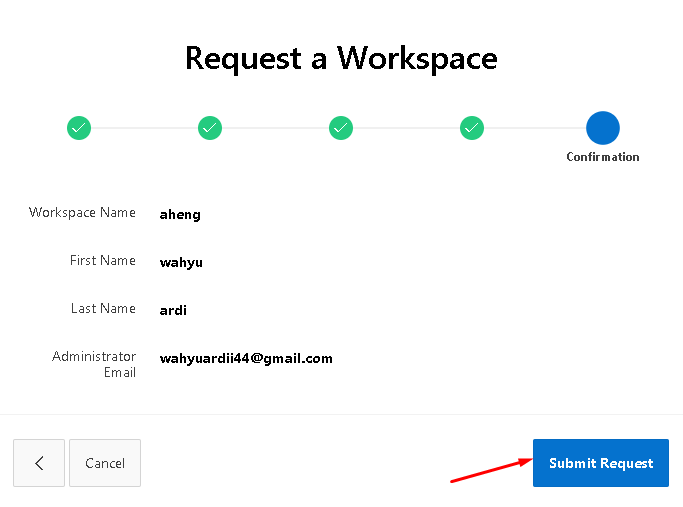
\includegraphics[width=5cm]{g.png}}
        \caption{\textit{confirmation}}
    \end{figure}

\item \textit{workspace requested}, kemudian buka gmail
    \begin{figure}[ht]
        \centerline{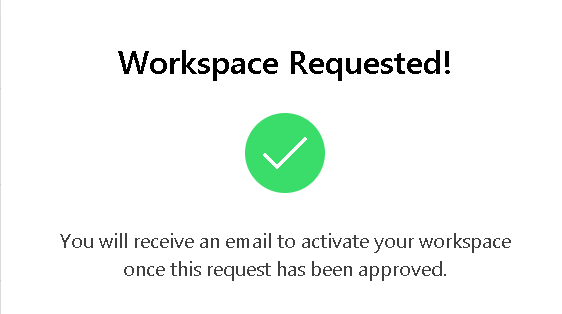
\includegraphics[width=5cm]{h.png}}
        \caption{\textit{workspace requested}}
    \end{figure}
    
\newpage

\item buka gmail, buka pesan dari oracle apex, kemudian klik \textit{create workspace}
     \begin{figure}[ht]
        \centerline{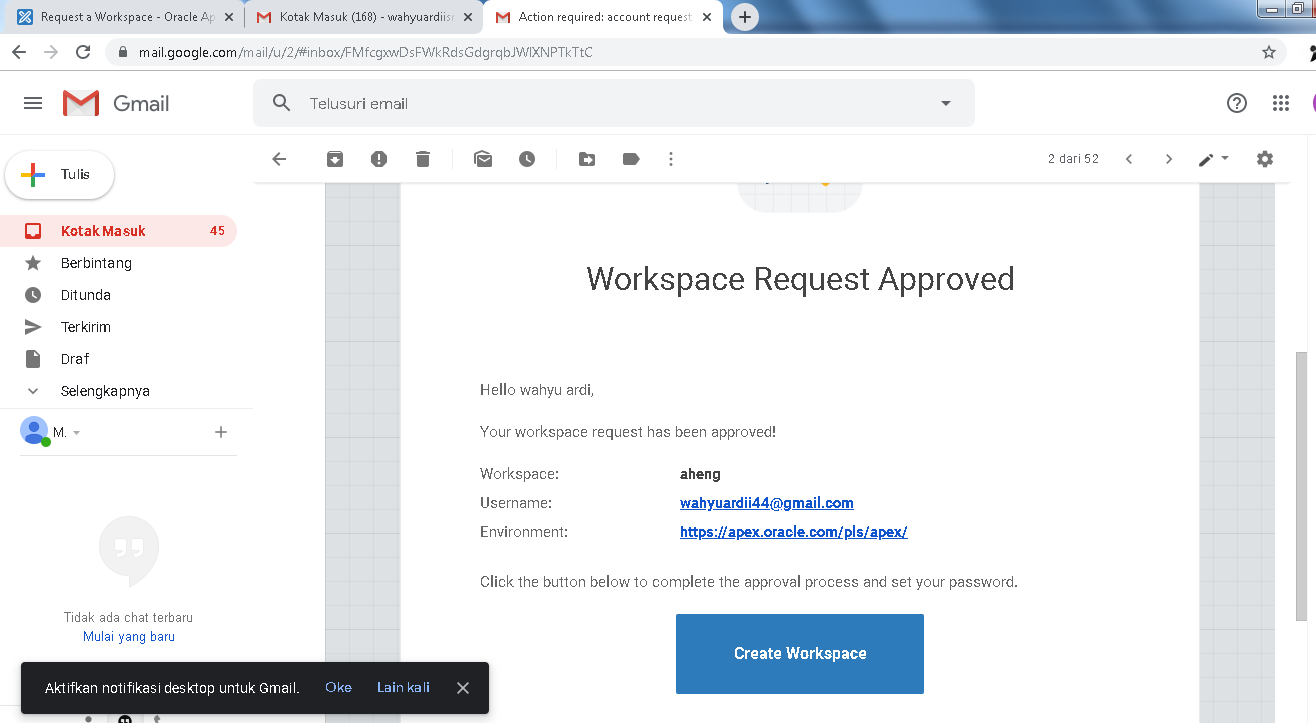
\includegraphics[width=5cm]{i.png}}
        \caption{\textit{create workspace}}
    \end{figure}

\item kemudian klik \textit{continue to sig in screen}
     \begin{figure}[ht]
        \centerline{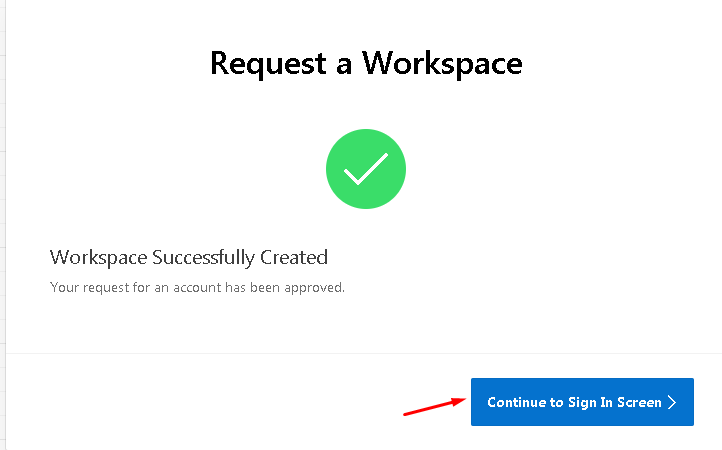
\includegraphics[width=4cm]{j.png}}
        \caption{\textit{continue to sig in screen}}
    \end{figure}

\item \textit{input new password} kemudian klik \textit{applychanges}
     \begin{figure}[ht]
        \centerline{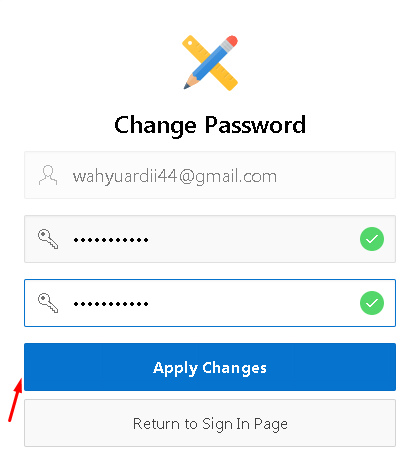
\includegraphics[width=4cm]{k.png}}
        \caption{\textit{applychanges}}
    \end{figure}
\end{enumerate}

\newpage

\subsection{Membuat Aplikasi di Oracle Apex}
\par Langkah-langkahnya yaitu:
\begin{enumerate}
\item login dengan \textit{akun oracle apex} anda
    \begin{figure}[ht]
        \centerline{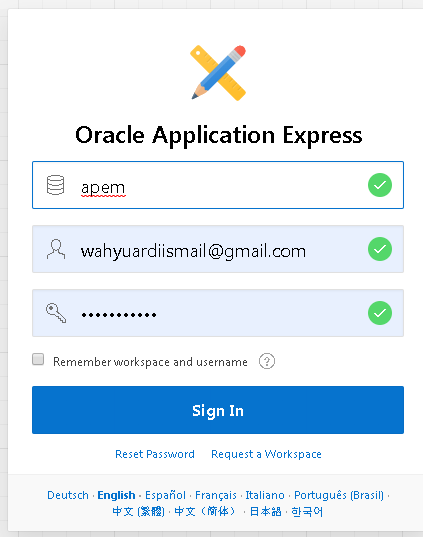
\includegraphics[width=4cm]{l.png}}
        \caption{\textit{login}}
    \end{figure}
    
\item klik \textit{app builder} 
     \begin{figure}[ht]
        \centerline{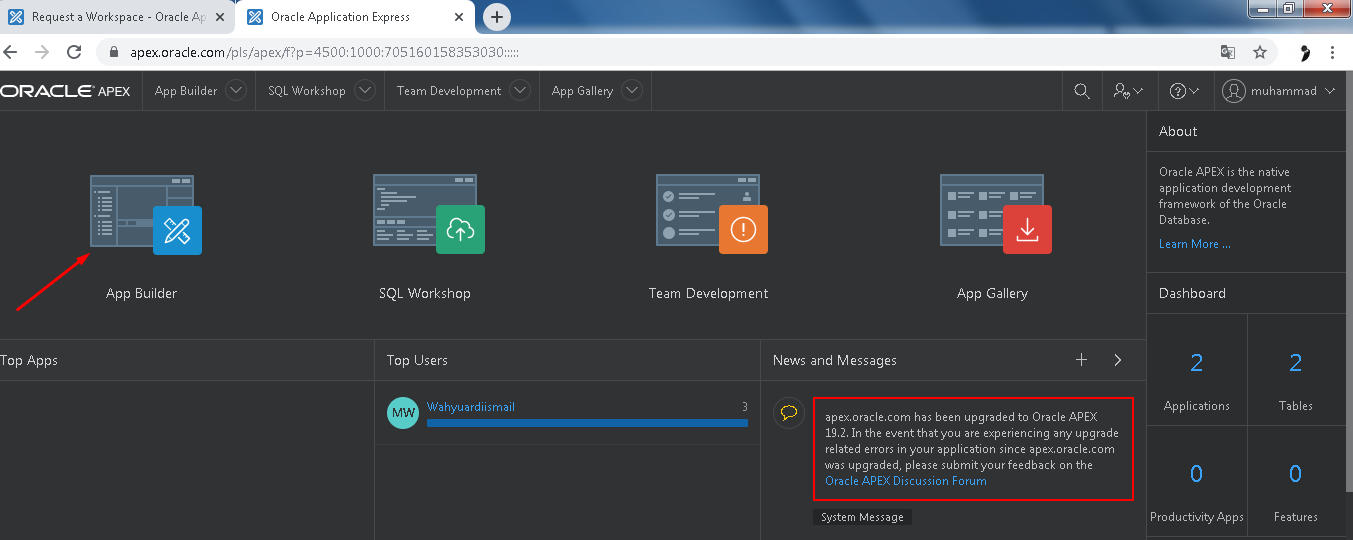
\includegraphics[width=4cm]{m.png}}
        \caption{\textit{app builder}}
    \end{figure}

\item klik create
     \begin{figure}[ht]
        \centerline{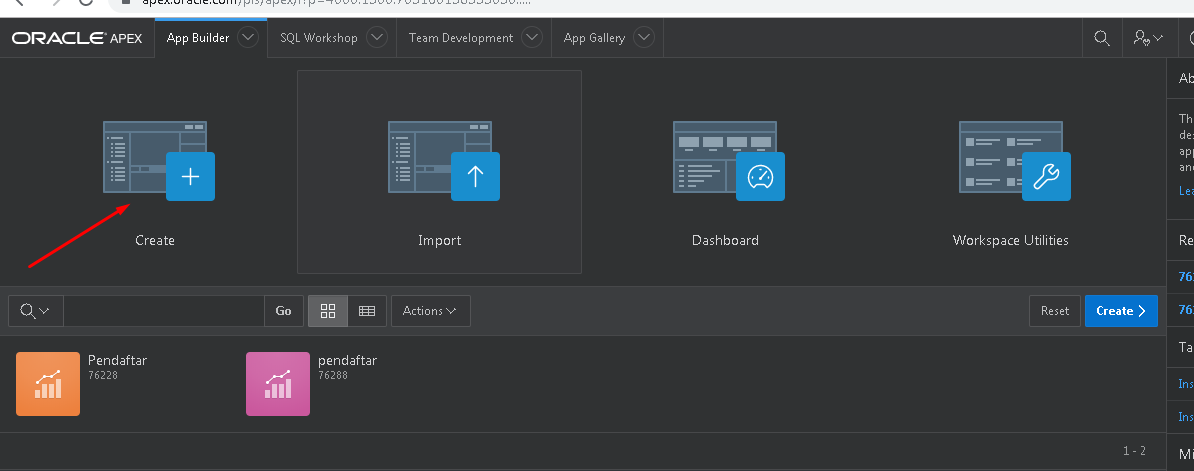
\includegraphics[width=4cm]{n.png}}
        \caption{\textit{create}}
    \end{figure}
    
\newpage

\item klik from a file, dengan format file microsoft excel nya csv
     \begin{figure}[ht]
        \centerline{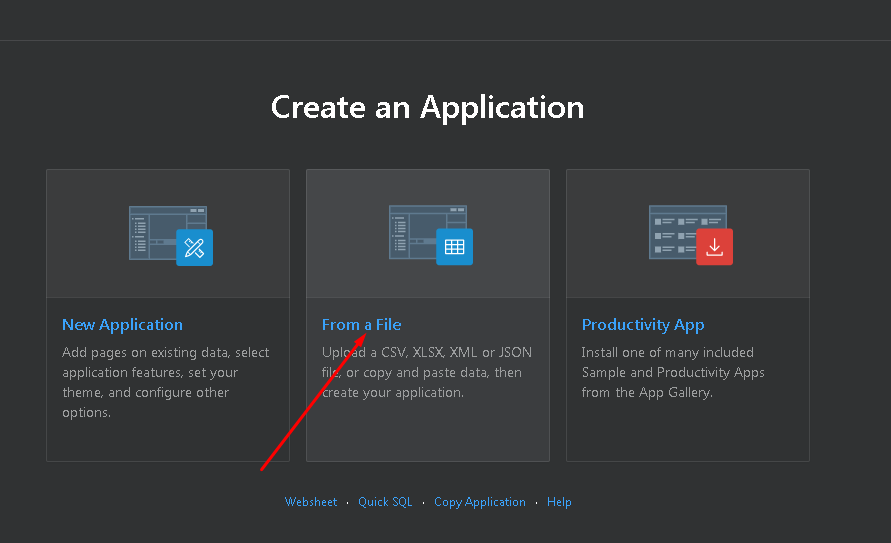
\includegraphics[width=4cm]{o.png}}
        \caption{\textit{from a file}}
    \end{figure}
    
\item masukin file excelnya dengan cara drag and drop
  \begin{figure}[ht]
        \centerline{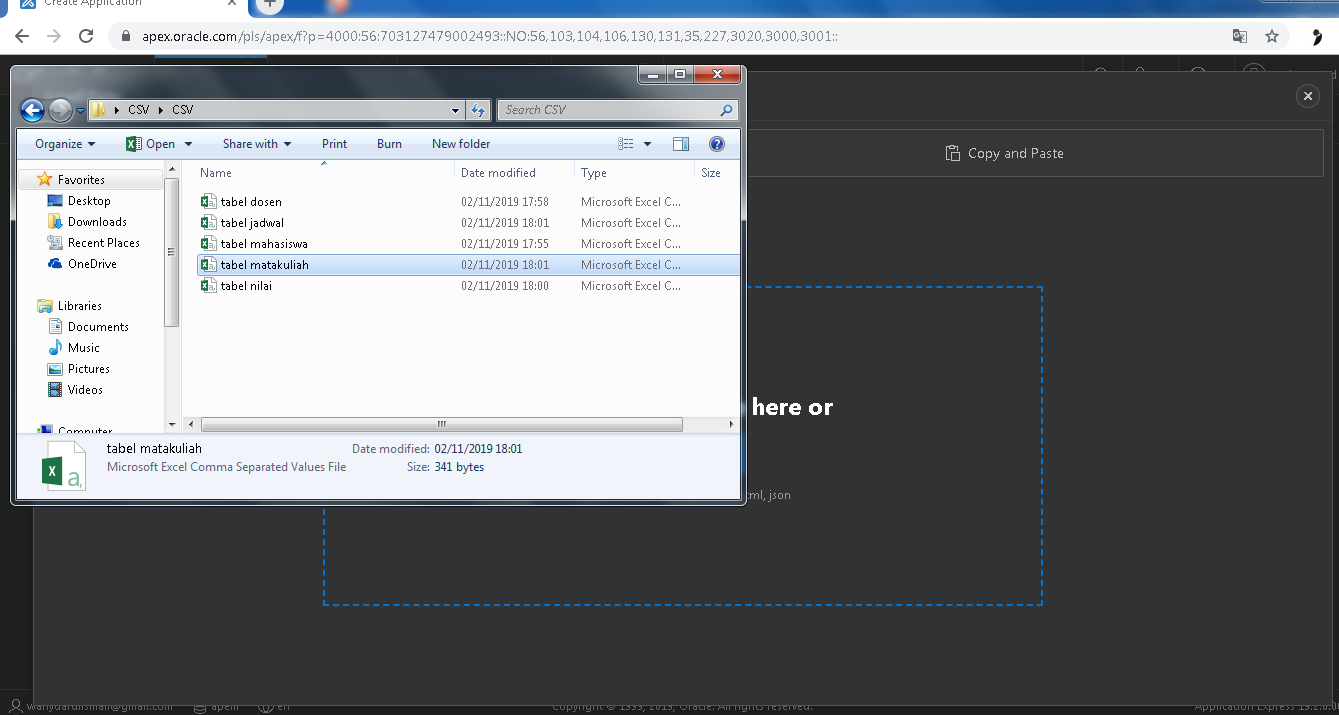
\includegraphics[width=4cm]{t.png}}
        \caption{\textit{drag and drop}}
    \end{figure}


  \begin{figure}[ht]
        \centerline{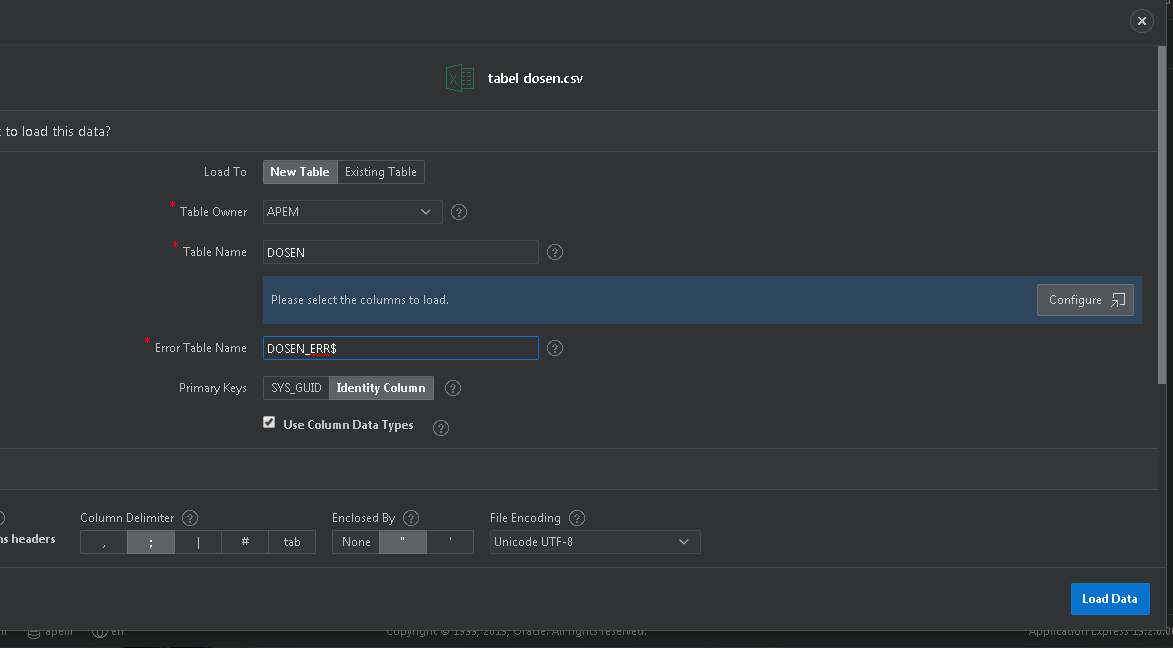
\includegraphics[width=4cm]{p.png}}
        \caption{\textit{tabeldosen}}
    \end{figure}

    \begin{figure}[ht]
        \centerline{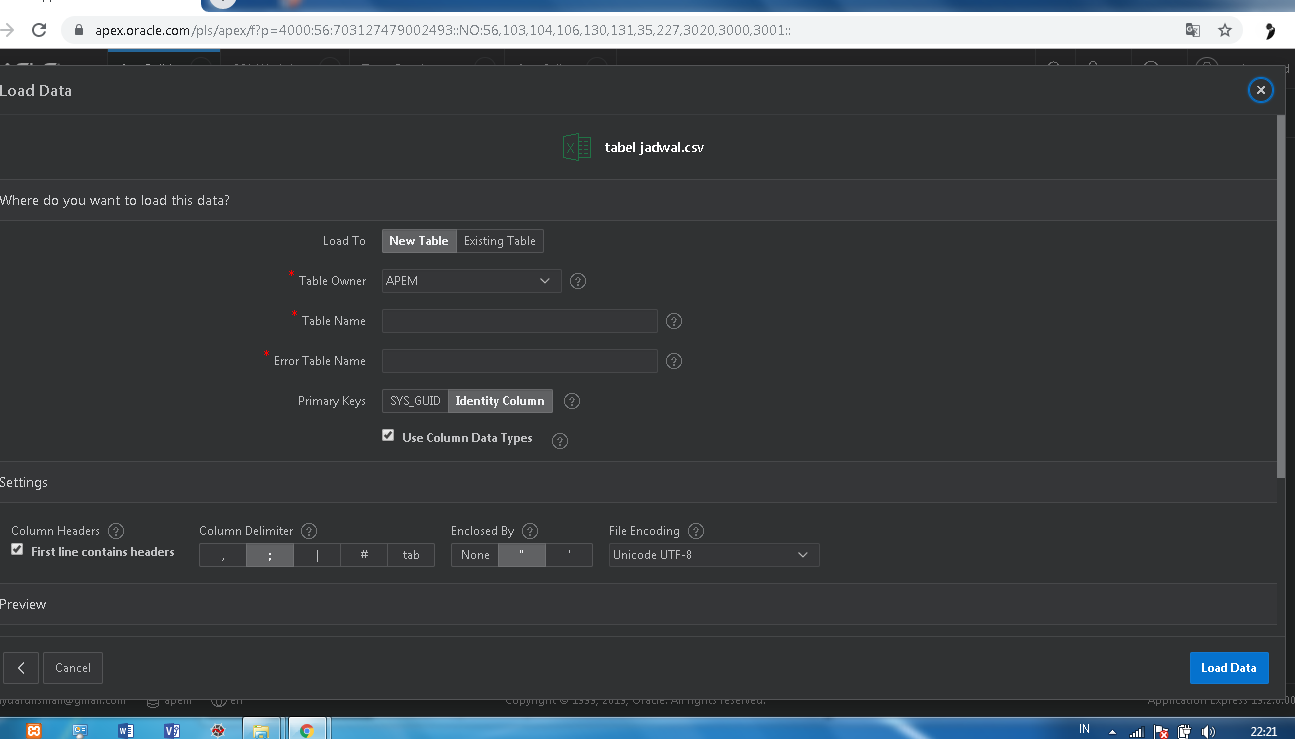
\includegraphics[width=4cm]{q.png}}
        \caption{\textit{tabeljadwal}}
    \end{figure}


    \begin{figure}[ht]
        \centerline{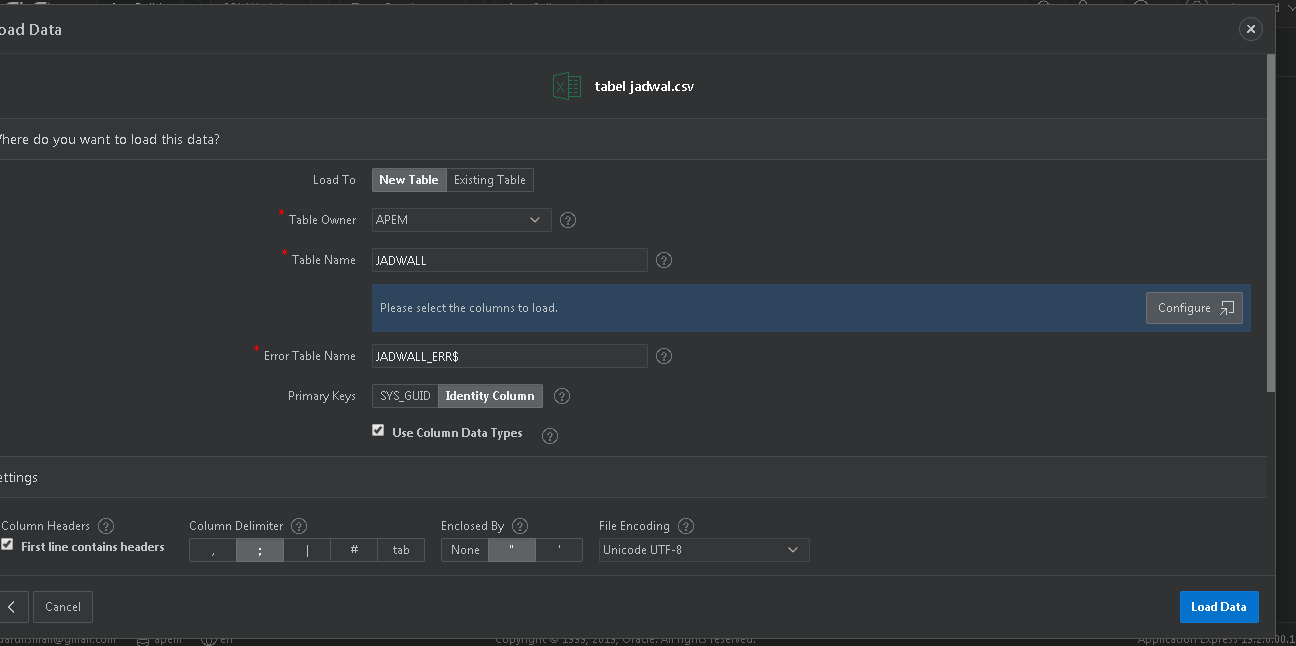
\includegraphics[width=4cm]{r.png}}
        \caption{\textit{tabeljadwal}}
    \end{figure}
    

    \begin{figure}[ht]
        \centerline{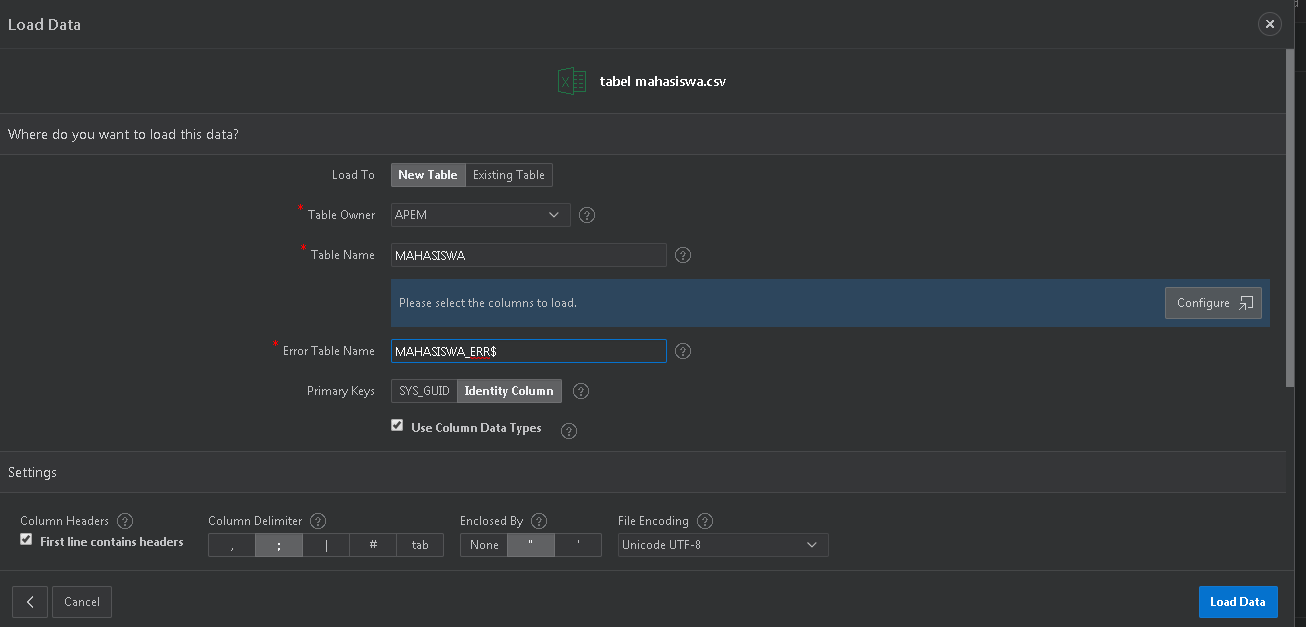
\includegraphics[width=4cm]{s.png}}
        \caption{\textit{tabelmahasiswa}}
    \end{figure}
    
\newpage
    \begin{figure}[ht]
        \centerline{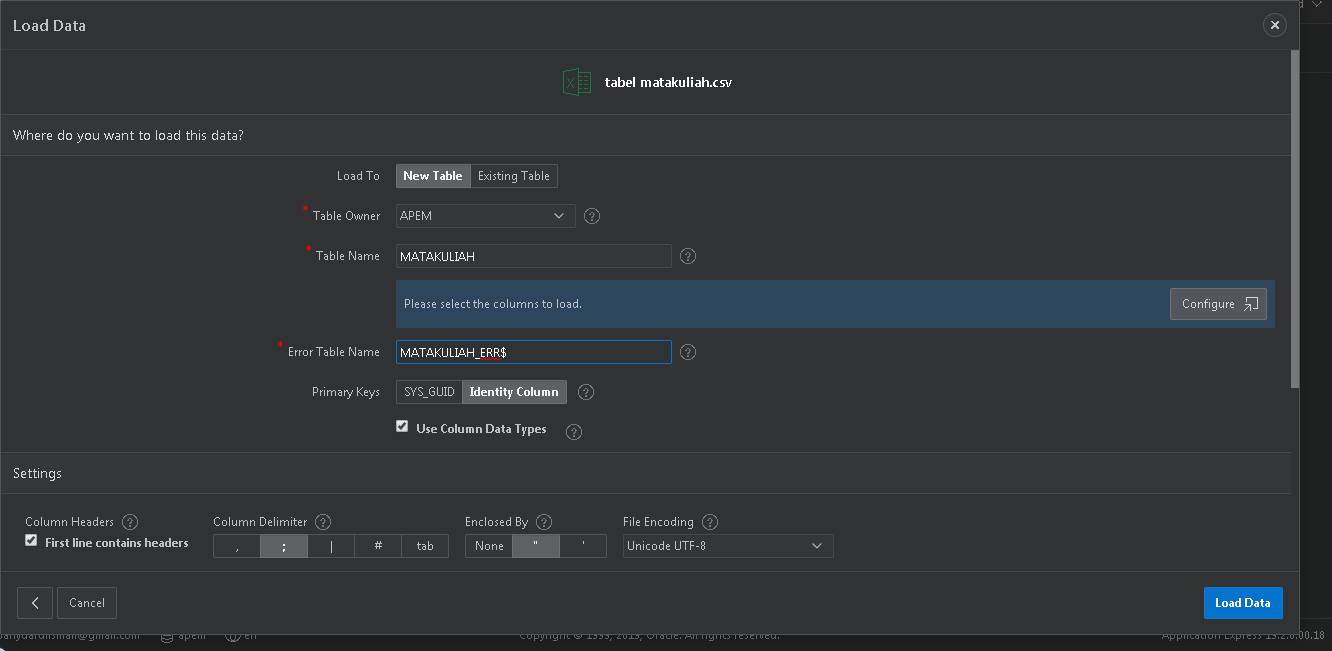
\includegraphics[width=4cm]{u.png}}
        \caption{\textit{tabelmatakuliah}}
    \end{figure}

\begin{figure}[ht]
        \centerline{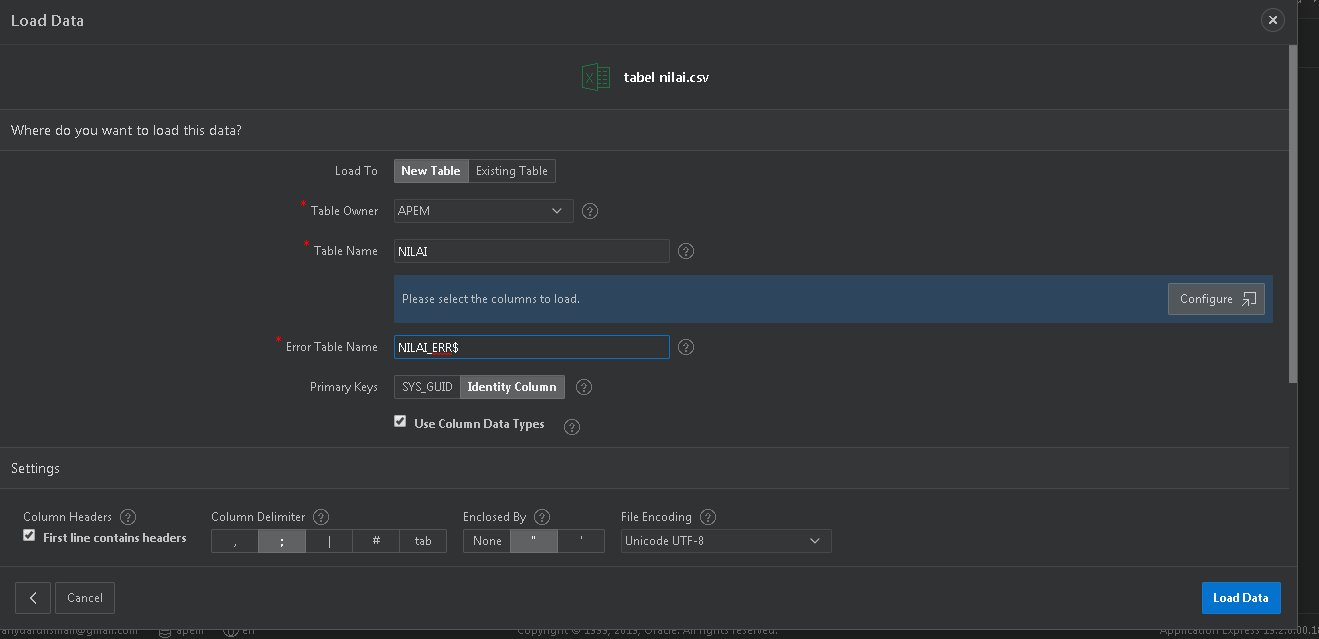
\includegraphics[width=4cm]{v.png}}
        \caption{\textit{tabelnilai}}
    \end{figure}   
    
\begin{figure}[ht]
        \centerline{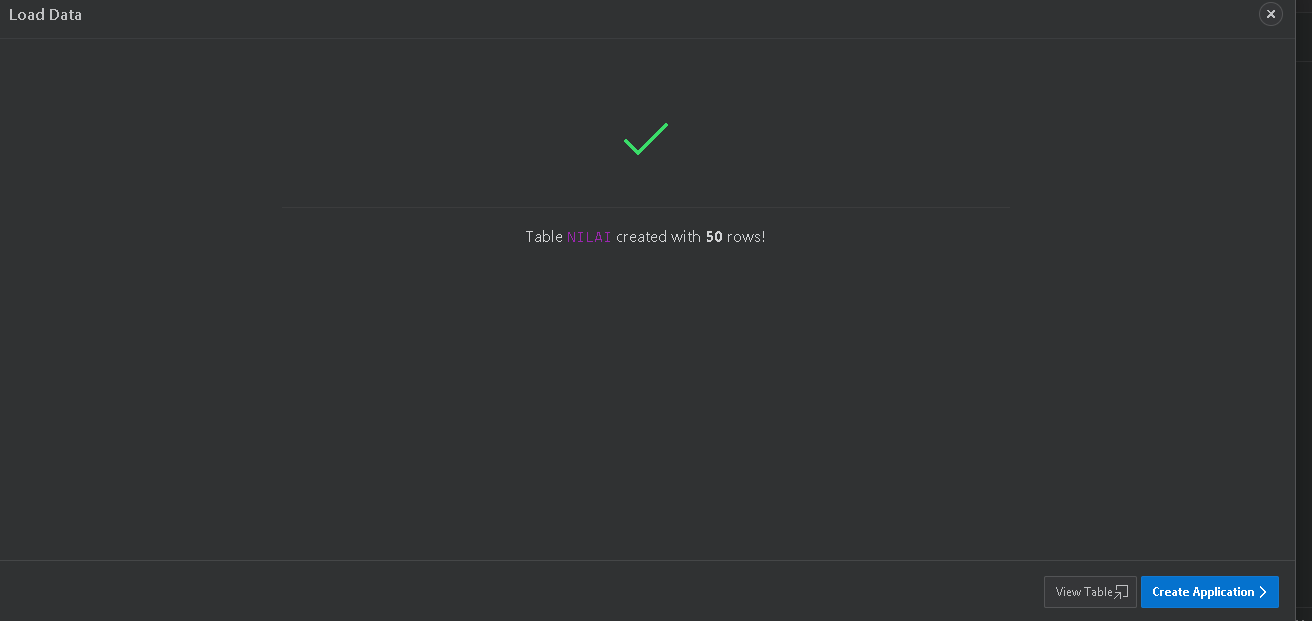
\includegraphics[width=4cm]{w.png}}
        \caption{\textit{klik create apllication}}
    \end{figure}

\newpage

\item create apllication dengan nama mahasiswapolpos
    \begin{figure}[ht]
        \centerline{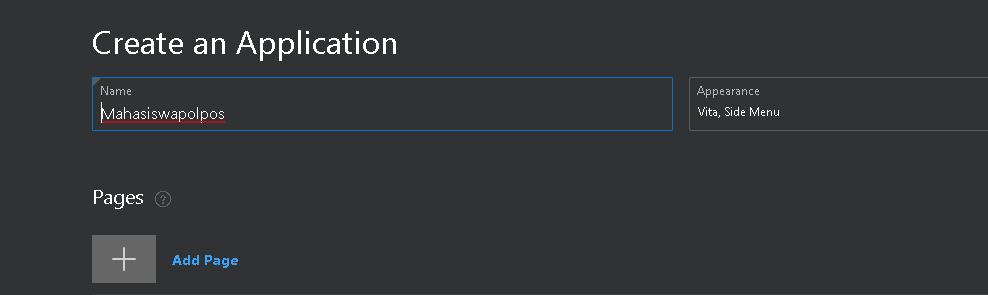
\includegraphics[width=4cm]{x.png}}
        \caption{\textit{create apllication}}
    \end{figure}

\item pilih interactive report 
    \begin{figure}[ht]
        \centerline{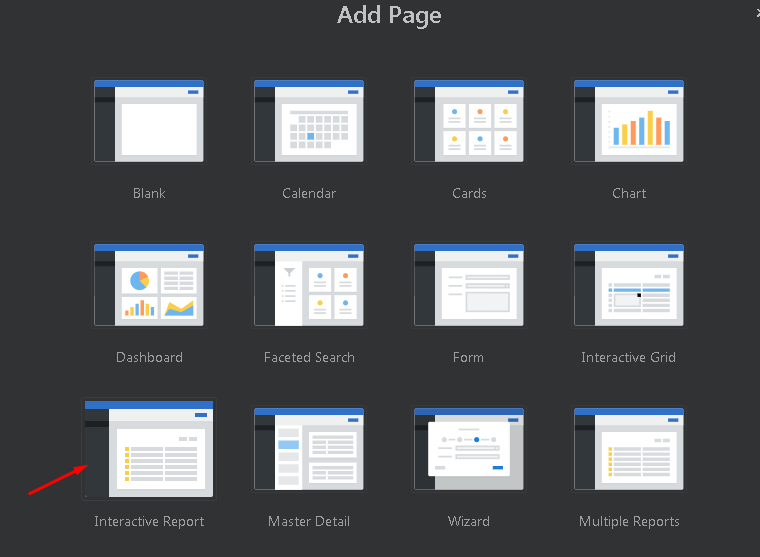
\includegraphics[width=4cm]{y.png}}
        \caption{\textit{interactive report}}
    \end{figure}

\item add report page
    \begin{figure}[ht]
        \centerline{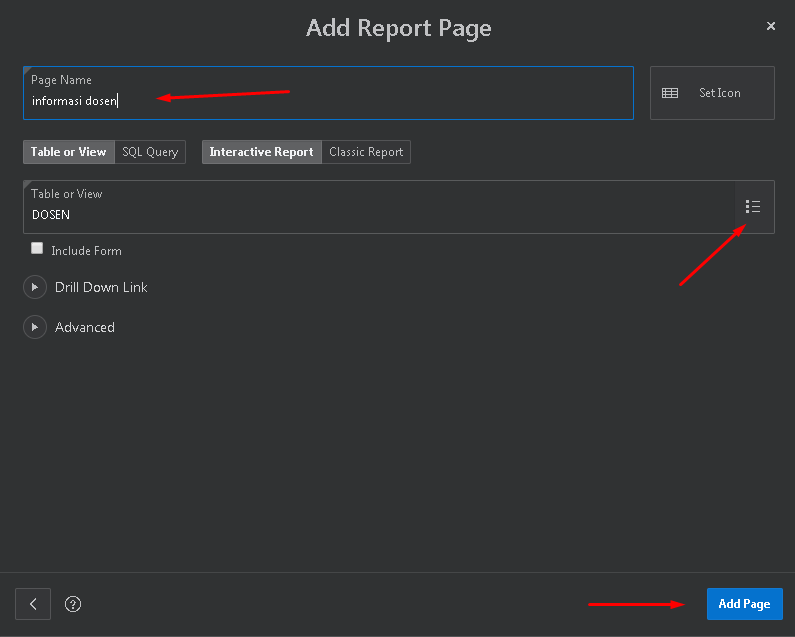
\includegraphics[width=4cm]{z.png}}
        \caption{\textit{add report pages}}
    \end{figure}

\item klik create apllication
    \begin{figure}[ht]
        \centerline{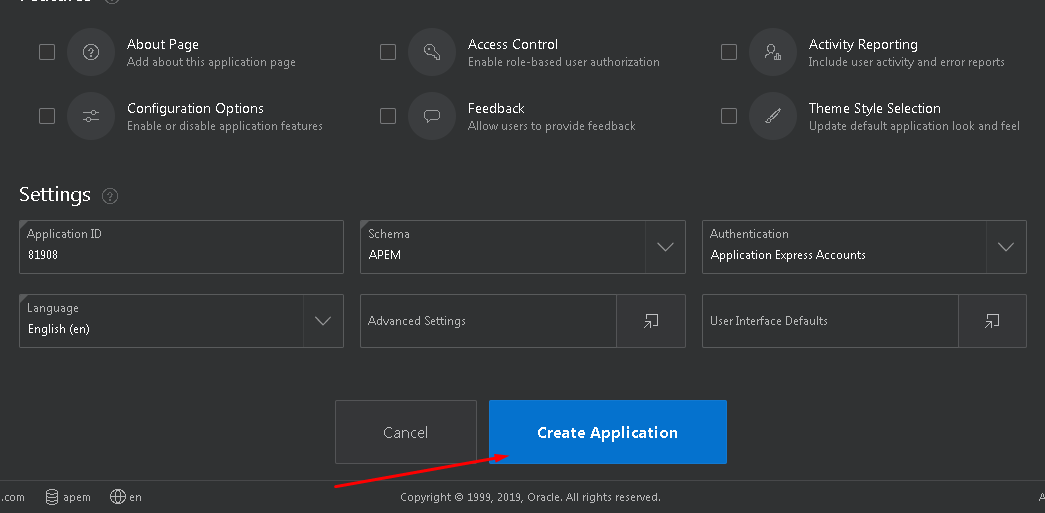
\includegraphics[width=4cm]{z1.png}}
        \caption{\textit{create apllication}}
    \end{figure}

\item login 
     \begin{figure}[ht]
        \centerline{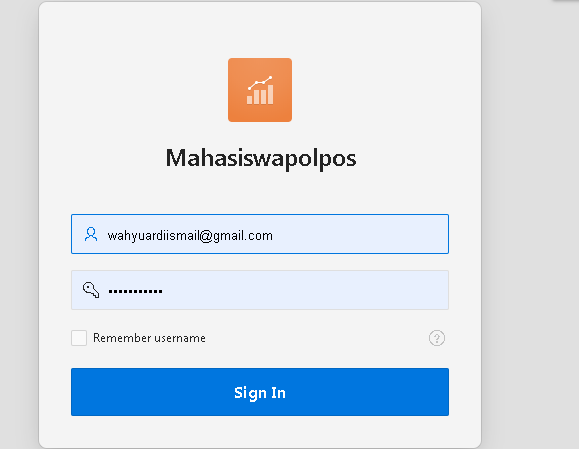
\includegraphics[width=4cm]{z2.png}}
        \caption{\textit{login}}
    \end{figure}

\item tampilan application
     \begin{figure}[ht]
        \centerline{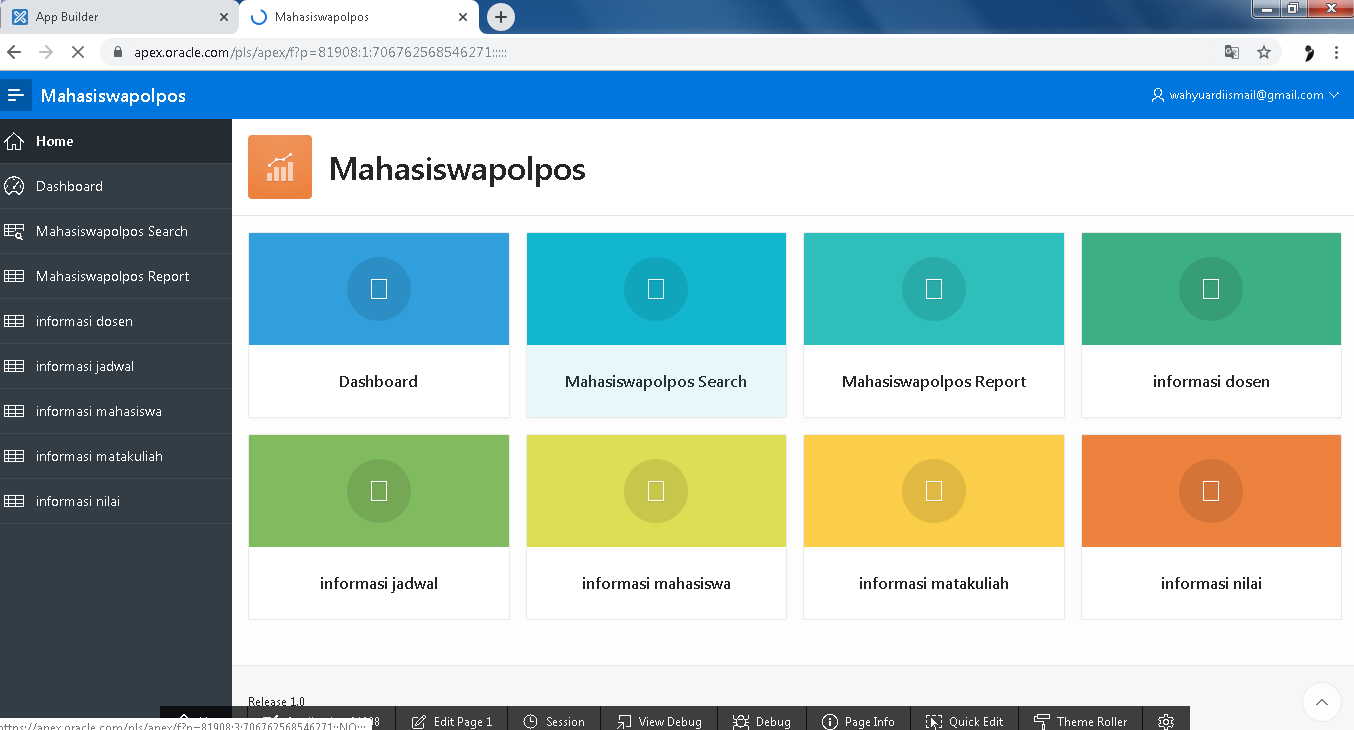
\includegraphics[width=4cm]{z3.png}}
        \caption{\textit{tampilan apllication}}
    \end{figure}
    
\newpage \\
workspace name :apem \\
first name     :muhammad \\
last name      :wahyu \\
administrator  :wahyuardiismail@gmail.com \\

\\
https://apex.oracle.com/pls/apex/f?p=81908:1:706762568546271:::::

\end{enumerate}


\end{document}
